\hypertarget{design-for-testability}{%
\section{Design for Testability}\label{design-for-testability}}

We just learned how the use of mocks and stubs can help developers in
being highly productive and efficient in writing test code. In our
previous chapter, it was easy to pass an \texttt{IssuedInvoices} stub to
the \texttt{InvoiceFilter} class. The refactoring operation we performed
(where we made the class receive its dependencies via constructors)
facilitated the testing of the \texttt{InvoiceFilter} class. Note,
however, that this was not the case at the beginning of that chapter. We
had to refactor the code for that to happen.

Software systems are often not ready/prepared to be tested, as seen in
the classes in our previous chapter. And so this chapter will show
\textbf{how to design and build a software system in a way that
increases its testability.}

Testability is the term used to describe how easy it is to write
automated tests for the system, class, or method to be tested. We
already know that automated tests are crucial for high-quality software;
it is, therefore, essential that our code is testable.

In this chapter, we'll discuss some design practices that increase the
testability of software systems. This idea is referred to as
\textbf{design for testability}. Specifically it involves:

\begin{itemize}
\tightlist
\item
  Dependency injection;
\item
  The separation between domain and infrastructure code;
\item
  Implementation-level tips.
\end{itemize}

\{\% set video\_id = ``iVJNaG3iqrQ'' \%\} \{\% include
``/includes/youtube.md'' \%\}

\hypertarget{dependency-injection}{%
\subsection{Dependency injection}\label{dependency-injection}}

Dependency injection is a design choice we can use to make our code more
testable. We will illustrate what dependency injection is by means of
this analogy:

\begin{quote}
We need a hammer to perform a certain task. When we are asked to do this
task, we find the hammer by ourselves and once we have the hammer, we
use it to perform the task. However, another approach is to say that,
while we still need a hammer when someone asks us to perform the task,
instead of getting the hammer ourselves, we get it from the person that
wants us to do the task.
\end{quote}

We can do the same when managing the dependencies in our systems. Simply
put, instead of the class instantiating the dependency itself, the class
asks for the dependency (via constructor or a setter, for example).

But let's revisit how we applied this idea in the previous chapter.
Let's assume that the \texttt{InvoiceFilter} was implemented as follows:

\begin{Shaded}
\begin{Highlighting}[]
\KeywordTok{public} \KeywordTok{class}\NormalTok{ InvoiceFilter \{}
 
  \KeywordTok{public} \DataTypeTok{void} \FunctionTok{filter}\NormalTok{() \{}
\NormalTok{    IssuedInvoices dao = }\KeywordTok{new} \FunctionTok{IssuedInvoices}\NormalTok{();}
 
    \CommentTok{// ...}
\NormalTok{  \}}
 
\NormalTok{\}}
\end{Highlighting}
\end{Shaded}

In our analogy, the \texttt{InvoiceFilter} (the worker) itself
instantiates (searches for) the \texttt{IssuedInvoices} (hammer) class.
With an implementation like this, there is no easy way to pass any mocks
to the \texttt{InvoiceFilter}. Any test code we devise will necessarily
use a concrete instance of \texttt{IssuedInvoices}. As we know,
\texttt{IssuedInvoices} goes to a database, which is something we have
been trying to avoid. Thus, we cannot control the way the
\texttt{IssuedInvoice} operates, at least for testing purposes. This
makes it harder for developers to write automated tests.

Instead, we can design our class in a way that it allows dependencies to
be injected. Note how we receive the dependency via constructor now:

\begin{Shaded}
\begin{Highlighting}[]
\KeywordTok{public} \KeywordTok{class}\NormalTok{ InvoiceFilter \{}
 
  \KeywordTok{private} \DataTypeTok{final}\NormalTok{ IssuedInvoices issuedInvoices;}
 
  \KeywordTok{public} \FunctionTok{InvoiceFilter}\NormalTok{(IssuedInvoices issuedInvoices) \{}
    \KeywordTok{this}\NormalTok{.}\FunctionTok{issuedInvoices}\NormalTok{ = issuedInvoices;}
\NormalTok{  \}}
 
  \KeywordTok{public} \DataTypeTok{void} \FunctionTok{lowValuedInvoices}\NormalTok{() \{}
    \CommentTok{// ...}
\NormalTok{  \}}
\NormalTok{\}}
\end{Highlighting}
\end{Shaded}

In this new implementation, we can now instantiate the
\texttt{InvoiceFilter} class and pass it a mocked/stubbed version of
\texttt{IssuedInvoices} in the test code. This simple change in the
design of the class makes the creation of automated tests easier and,
therefore, increases the testability of the code.

Note that with such a design decision, the \texttt{InvoiceFilter} class
also enables the production code to pass a concrete instance of
\texttt{IssueInvoices}. After all, when the program is running ``for
real'', we want the real implementation of \texttt{IssuedInvoices} to
work.

More formally, \emph{Dependency injection} is a technique where one
object supplies the required dependencies of the another object. As in
our example, whenever a client decides to make use of
\texttt{InvoiceFilter}, it will have to also supply an
\texttt{IssuedInvoice}. The term ``injection'' is about ``injecting'' a
dependency, in this case the \texttt{IssuedInvoice}, to another class,
in this case \texttt{InvoiceFilter}.

The use of dependency injection improves our code in many ways:

\begin{itemize}
\tightlist
\item
  It enables us to mock/stub the dependencies in the test code,
  increasing the productivity of the developer during the testing phase.
\item
  It makes all the dependencies more explicit; after all, they all need
  to be injected (via constructor, for example).
\item
  It affords better separation of concerns: classes now do not need to
  worry about how to build their dependencies, as they are injected to
  them.
\item
  The class becomes more extensible. As a client of the class, you can
  pass any dependency via the constructor. Suppose a class depends on a
  type \texttt{A} (and receives it via constructor). As a client, you
  can pass \texttt{A} or any implementation of \texttt{A}, e.g., if
  \texttt{A} is \texttt{List}, you can pass \texttt{ArrayList} or
  \texttt{LinkedList}. Your class can now work with many different
  implementations of \texttt{A}.
\end{itemize}

\{\% hint style=`tip'\%\} If you want to understand more advanced OOP
concepts, we suggest reading more about:

\begin{itemize}
\tightlist
\item
  The Open-Closed Principle;
\item
  Inversion of Control;
\item
  Separation of concerns. \{\% endhint \%\}
\end{itemize}

\{\% set video\_id = ``mGdsdBEWB5E'' \%\} \{\% include
``/includes/youtube.md'' \%\}

\hypertarget{domain-vs-infrastructure}{%
\subsection{Domain vs infrastructure}\label{domain-vs-infrastructure}}

A general recommendation to design for testability comes down to
separating \emph{domain} from \emph{infrastructure}. The \emph{domain}
is where the core of the system lies, i.e.~where all the business rules,
logics, entities, services, etc, reside. Throughout this book we have
been using business systems as examples. Entities like \texttt{Invoice},
\texttt{ChristmasDiscountCalculator} are examples of domain classes.

\emph{Infrastructure} relates to all code that handles some
infrastructure. For example, pieces of code that handle database
queries, or webservice calls, or file reads and writes. In our examples,
all our Data Access Objects are part of what we call infrastructure
code.

We observe that, when domain code and infrastructure code are mixed up
together, the system becomes harder to test. Let us go back to our
\texttt{InvoiceFilter} example with it now containing the SQL logic,
instead of it depending on a Data Access Object:

\begin{Shaded}
\begin{Highlighting}[]
\KeywordTok{public} \KeywordTok{class}\NormalTok{ InvoiceFilter \{}
 
  \CommentTok{// accessing the database}
  \KeywordTok{private} \BuiltInTok{List}\NormalTok{\textless{}IssuedInvoice\textgreater{} }\FunctionTok{all}\NormalTok{() \{}
    \BuiltInTok{Connection}\NormalTok{ connection = }\BuiltInTok{DriverManager}\NormalTok{.}\FunctionTok{getConnection}\NormalTok{(}\StringTok{"db"}\NormalTok{, }\StringTok{"root"}\NormalTok{, }\StringTok{""}\NormalTok{);}
 
    \KeywordTok{return} \FunctionTok{withSql}\NormalTok{( () {-}\textgreater{} \{}
        \KeywordTok{try}\NormalTok{ (var ps = connection.}\FunctionTok{prepareStatement}\NormalTok{(}\StringTok{"select * from invoice"}\NormalTok{)) \{}
            \DataTypeTok{final}\NormalTok{ var rs = ps.}\FunctionTok{executeQuery}\NormalTok{();}
 
            \BuiltInTok{List}\NormalTok{\textless{}Invoice\textgreater{} allInvoices = }\KeywordTok{new} \BuiltInTok{ArrayList}\NormalTok{\textless{}\textgreater{}();}
            \KeywordTok{while}\NormalTok{ (rs.}\FunctionTok{next}\NormalTok{()) \{}
\NormalTok{                allInvoices.}\FunctionTok{add}\NormalTok{(}\KeywordTok{new} \FunctionTok{Invoice}\NormalTok{(rs.}\FunctionTok{getString}\NormalTok{(}\StringTok{"name"}\NormalTok{), rs.}\FunctionTok{getInt}\NormalTok{(}\StringTok{"value"}\NormalTok{)));}
\NormalTok{            \}}
            \KeywordTok{return}\NormalTok{ allInvoices;}
\NormalTok{        \}}
\NormalTok{    \});}
 
\NormalTok{    connection.}\FunctionTok{close}\NormalTok{();}
\NormalTok{  \}}
 
  \KeywordTok{public} \BuiltInTok{List}\NormalTok{\textless{}Invoice\textgreater{} }\FunctionTok{lowValueInvoices}\NormalTok{() \{}
 
\NormalTok{    var issuedInvoices = }\FunctionTok{all}\NormalTok{();}
 
    \KeywordTok{return}\NormalTok{ issuedInvoices.}\FunctionTok{all}\NormalTok{().}\FunctionTok{stream}\NormalTok{()}
\NormalTok{        .}\FunctionTok{filter}\NormalTok{(invoice {-}\textgreater{} invoice.}\FunctionTok{value}\NormalTok{ \textless{} }\DecValTok{100}\NormalTok{)}
\NormalTok{        .}\FunctionTok{collect}\NormalTok{(}\FunctionTok{toList}\NormalTok{());}
\NormalTok{  \}}
 
\NormalTok{\}}
\end{Highlighting}
\end{Shaded}

We can make the following observations about the code above:

\begin{itemize}
\tightlist
\item
  The code is less cohesive. It knows how to extract data from the
  database and it also knows the ``low value invoices'' business rule.
  This class now requires test cases that cover both responsibilities.
\item
  Domain code and infrastructure code are mixed up. This means a tester
  will not be able to avoid database access when testing the ``low value
  invoices'' rule. As we have seen many times already, this will incur
  higher costs.
\item
  This new version of the \texttt{InvoiceFilter} class is definitely
  more complex than our previous version and complex code are more prone
  to defects.
\end{itemize}

Our previous version was indeed better. It was more cohesive and
simpler. More importantly it also had a clear separation between domain
code and infrastructure code. This is what software developers should
always do when they design systems in order to ensure these two
responsibilities are separated from each other.

This idea of separating infrastructure and domain is explored in the
following literature:

\begin{itemize}
\tightlist
\item
  In the \textbf{Ports and Adapters} (also called the \textbf{Hexagonal
  Architecture}) idea, as proposed by Alistair Cockburn, the domain
  (business logic) depends on ``Ports'', rather than directly on the
  infrastructure. These ports are interfaces that define what the
  infrastructure is able to do. These ports are completely separated
  from the implementation of the infrastructure. The ``adapters'', on
  the other hand, are very close to the infrastructure. These are the
  implementations of the ports that talk to the database, webservice,
  etc. They know how the infrastructure works and how to communicate
  with it.
\end{itemize}

In the schema below, you can see that the ports are part of the domain.

\begin{figure}
\centering
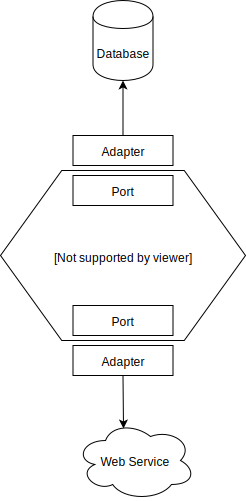
\includegraphics{img/design-for-testability/hexagonal_architecture.svg}
\caption{Hexagonal Architecture}
\end{figure}

Ports and Adapters help us a lot with the testability of our code. If
our core domain depends only on ports, we can easily stub/mock them.

\begin{itemize}
\tightlist
\item
  In his \textbf{Domain-Driven Design} work, Eric Evans proposes that
  the domain (the core of the system) will be isolated from the
  infrastructure layer. Besides all the design benefits that Eric cites
  in his book, testers benefit from this separation, as it enables them
  to exercise parts of code without having to depend on heavy
  infrastructure.
\end{itemize}

In practice, we observe that separating the infrastructure from domain
is often challenging. The database example, where we move all the code
to another class, is rather a simplistic one. When building software, we
frequently rely on different libraries and frameworks that are often
opinionated and require you to follow certain design decisions that
might not be ideal, from a testability perspective. It is the duty of a
developer to be able to abstract these problems, making sure that the
domain concerns are always separated from the infrastructure concerns.

\{\% hint style=`tip' \%\} You see developers vouching for domain
objects not to depend on concrete implementations of the infrastructure
code, but rather, to depend solely on abstractions. In our example, the
\texttt{InvoiceFilter} domain object, instead of depending on a concrete
implementation of \texttt{IssuedInvoices} (one that right now contains
SQL code and knows how to communicate with the database), it would
depend on an abstraction/interface.

By devising interfaces that represent the abstract interaction that
domains and infrastructure classes will have with each other, the
developer ends up separating the concerns in a better way, reducing the
coupling between both layers, and devising simpler flows of interactions
between both layers.

The dependency inversion principle (note the \emph{inversion} and not
\emph{injection}) helps us to formalise these concepts:

\begin{itemize}
\tightlist
\item
  High-level modules should not depend on low-level modules. Both should
  depend on abstractions (e.g.~interfaces).
\item
  Abstractions should not depend on details. Details (concrete
  implementations) should depend on abstractions. \{\% endhint \%\}
\end{itemize}

\{\% set video\_id = ``hv1XV87lJgA'' \%\} \{\% include
``/includes/youtube.md'' \%\}

\hypertarget{implementation-level-tips-on-designing-for-testability}{%
\subsection{Implementation-level tips on designing for
testability}\label{implementation-level-tips-on-designing-for-testability}}

We end this chapter with a couple of practical tips that will help you
to devise testable systems/classes:

\begin{itemize}
\item
  \textbf{Cohesion and testability}: cohesive classes are classes that
  do only one thing. Cohesive classes tend to be easier to test. This is
  because fewer responsibilities imply fewer test cases and fewer
  responsibilities often imply fewer dependencies (as you need fewer to
  compose the required functionality) which in turn incurs lower testing
  costs. On the other hand, a non-cohesive class tends to consume a
  large amount of testing effort from developers. You might notice that
  a non-cohesive class requires so many test cases, that you often feel
  like ``the testing is never-ending''. Refactoring non-cohesive classes
  is therefore an important task when it comes to testability. A common
  way to do this is by splitting the non-cohesive class into several
  smaller-but-cohesive classes. Each small class can then be tested
  separately, and the class that combines them might rely either on mock
  objects to assert the correctness of the interactions among the
  dependencies or on an integration test (or both).
\item
  \textbf{Coupling and testability}: Coupling refers to the number of
  classes that a class depends on. A highly coupled class requires
  several other classes to do its work. Coupling decreases testability.
  A tester trying to test a highly dependent class ends up having to
  test all its dependencies together. If the tester then decides to use
  stubs/mocks, the costs of setting them up will also be higher than it
  needed to be (just imagine yourself setting up 10 or 15 stubs/mocks to
  test a single class). Moreover, the number of test cases that would be
  required to achieve a minimum amount of coverage is too high, as each
  dependency probably brings together a whole set of requirements and
  conditions. Reducing coupling, however, is often tricky, and maybe one
  of the biggest challenges in software design. A common
  coupling-related refactoring is to group dependencies together into a
  higher and meaningful abstraction. Imagine that class A depends on B,
  C, D and E. After inspection, you notice that B interacts with C, and
  D interacts with E. Devising a new class that handles the
  communication between B and C (let us call it BC), and other one that
  handles the communication between D and E (let us call it DE), already
  reduces A's coupling. After all, it now depends only on BC, and DE. In
  general, pushing responsibilities and dependencies to smaller classes
  and later connecting them via larger abstractions is the way to go.
\item
  \textbf{Complex conditions and testability}: We have seen in previous
  chapters that conditions that are very complex (e.g., an \texttt{if}
  statement composed of multiple Boolean operations) require great
  effort from testers. For example, the number of tests one might devise
  after applying some boundary testing or condition+branch coverage
  criteria might be too high. Reducing the complexity of such
  conditions, for example by breaking it into multiple smaller
  conditions, will not reduce the overall complexity of the problem, but
  will ``spread'' it.
\item
  \textbf{Private methods and testability}: A common question among
  developers is whether to test private methods or not. In principle,
  testers should test private methods only through their public methods.
  However, testers often feel the urge to test a particular private
  method in isolation. One common cause for this feeling is the lack of
  cohesion or the complexity of this private method. In other words,
  this method does something so different to the public method, and/or
  its task is so complex, that it has to be tested separately. This is a
  good example of when ``the test speaks to the developer'' (a common
  saying among Test-Driven Developers). In terms of the design this
  might mean that this private method does not belong in its current
  place. A common refactoring is to extract this method, maybe to a
  brand new class. There, the former private method, now a public
  method, can be tested normally by the developer. The original class,
  where the private method used to be, should now depend on this new
  class.
\item
  \textbf{Static methods and testability}: As we have seen before,
  static methods adversely affect testability, as they can not be
  stubbed easily. Therefore, a good rule of thumb is to avoid the
  creation of static methods whenever possible. Exceptions to this rule
  are utility methods. As we saw before, utility methods are often not
  mocked. If your system has to depend on a specific static method,
  e.g., because it comes with the framework your software depends on,
  adding an abstraction on top of it, similar to what we did with the
  \texttt{Calendar} class in the previous chapter, might be a good
  decision to facilitate testability. The same recommendation applies
  when your system needs code from others or external dependencies.
  Again, creating layers/classes that abstract away the dependency might
  help you in increasing testability. We emphasise that developers
  should not be afraid to create these extra layers. While it might seem
  that these layers will increase the overall complexity of the design,
  the increased testability pays off.
\end{itemize}

Finally, note how there is a
\href{https://www.youtube.com/watch?v=4cVZvoFGJTU}{deep synergy between
well designed production code and testability}. We repeat that focusing
only on testing techniques (like the ones we discussed in the
\emph{Testing Techniques} section of this book), or only on design
techniques (like the ones we have been focusing on in this section of
the book), is not enough. High-quality software is only achieved when
software systems are designed with testability in mind, and rigorous
testing techniques are applied.

\{\% set video\_id = ``VaScxLhsDBQ'' \%\} \{\% include
``/includes/youtube.md'' \%\}

\hypertarget{exercises}{%
\subsection{Exercises}\label{exercises}}

\textbf{Exercise 1.} How can we improve the testability of the
\texttt{OrderDeliveryBatch} class?

\begin{Shaded}
\begin{Highlighting}[]
\KeywordTok{public} \KeywordTok{class}\NormalTok{ OrderDeliveryBatch \{}
 
  \KeywordTok{public} \DataTypeTok{void} \FunctionTok{runBatch}\NormalTok{() \{}
 
\NormalTok{    OrderDao dao = }\KeywordTok{new} \FunctionTok{OrderDao}\NormalTok{();}
\NormalTok{    DeliveryStartProcess delivery = }\KeywordTok{new} \FunctionTok{DeliveryStartProcess}\NormalTok{();}
 
    \BuiltInTok{List}\NormalTok{\textless{}Order\textgreater{} orders = dao.}\FunctionTok{paidButNotDelivered}\NormalTok{();}
 
    \KeywordTok{for}\NormalTok{ (Order order : orders) \{}
\NormalTok{      delivery.}\FunctionTok{start}\NormalTok{(order);}
 
      \KeywordTok{if}\NormalTok{ (order.}\FunctionTok{isInternational}\NormalTok{()) \{}
\NormalTok{        order.}\FunctionTok{setDeliveryDate}\NormalTok{(}\StringTok{"5 days from now"}\NormalTok{);}
\NormalTok{      \} }\KeywordTok{else}\NormalTok{ \{}
\NormalTok{        order.}\FunctionTok{setDeliveryDate}\NormalTok{(}\StringTok{"2 days from now"}\NormalTok{);}
\NormalTok{      \}}
\NormalTok{    \}}
\NormalTok{  \}}
\NormalTok{\}}
 
\KeywordTok{class}\NormalTok{ OrderDao \{}
  \CommentTok{// accesses a database}
\NormalTok{\}}
 
\KeywordTok{class}\NormalTok{ DeliveryStartProcess \{}
  \CommentTok{// communicates with a third{-}party webservice}
\NormalTok{\}}
\end{Highlighting}
\end{Shaded}

Which techniques can we apply? What would the new implementation look
like? Think about what you would need to include in order to test the
\texttt{OrderDeliveryBatch} class.

\textbf{Exercise 2.} Consider the following requirement and
implementation.

\begin{verbatim}
A webshop gives a discount of 15% on King's Day.
\end{verbatim}

\begin{Shaded}
\begin{Highlighting}[]
\KeywordTok{public} \KeywordTok{class}\NormalTok{ KingsDayDiscount \{}
 
  \KeywordTok{public} \DataTypeTok{double} \FunctionTok{discount}\NormalTok{(}\DataTypeTok{double}\NormalTok{ value) \{}
 
    \BuiltInTok{Calendar}\NormalTok{ today = }\BuiltInTok{Calendar}\NormalTok{.}\FunctionTok{getInstance}\NormalTok{();}
 
    \DataTypeTok{boolean}\NormalTok{ isKingsDay = today.}\FunctionTok{get}\NormalTok{(MONTH) == }\BuiltInTok{Calendar}\NormalTok{.}\FunctionTok{APRIL}
\NormalTok{        \&\& today.}\FunctionTok{get}\NormalTok{(DAY\_OF\_MONTH) == }\DecValTok{27}\NormalTok{;}
 
    \KeywordTok{return}\NormalTok{ isKingsDay ? value * }\FloatTok{0.}\DecValTok{15}\NormalTok{ : }\DecValTok{0}\NormalTok{;}
 
\NormalTok{  \}}
\NormalTok{\}}
\end{Highlighting}
\end{Shaded}

We want to create a unit test for this class.

Why does this class have bad testability? What can we do to improve the
testability? I.e. why is it difficult to test the method?

\textbf{Exercise 3.} Sarah has joined a mobile app team that has been
trying to write automated tests for a while. The team wants to write
unit tests for part of their code, but ``that's really hard'', according
to the developers.

After some code review, the developers themselves listed the following
problems in their codebase:

\begin{enumerate}
\def\labelenumi{\arabic{enumi}.}
\tightlist
\item
  Many classes mix infrastructure and business rules
\item
  The database has large tables and no indexes
\item
  Use of static methods
\item
  Some classes have too many attributes/fields
\end{enumerate}

To increase the testability, the team has a budget to work on two out of
the four issues above. Which items should Sarah recommend them to tackle
first?

Note: All of the four issues should obviously be fixed. However, try to
prioritise the two most important ones: which influence the testability
the most?

\textbf{Exercise 4.} Observability and controllability are two important
concepts when it comes to software testing. Three developers could
benefit from improving either the observability or the controllability
of the system/class which they are testing but each developer encounters
a problem:

\begin{enumerate}
\def\labelenumi{\arabic{enumi}.}
\tightlist
\item
  ``I can't really assert that the method under test worked well.''
\item
  ``I need to make sure this class starts with that Boolean set to
  false, but I simply can't do it.''
\item
  ``I just instantiated the mock object, but there's no way to inject it
  in the class.''
\end{enumerate}

State for each of the problems above whether it relates to observability
or controllability.

\hypertarget{references}{%
\subsection{References}\label{references}}

\begin{itemize}
\item
  Cockburn, Alistair. The Hexagonal Architecture.
  https://wiki.c2.com/?HexagonalArchitecture
\item
  Hevery, Misko. The Testability Guide.
  http://misko.hevery.com/attachments/Guide-Writing\%20Testable\%20Code.pdf
\item
  Michael Feathers. The deep synergy between well design production code
  and testability. https://www.youtube.com/watch?v=4cVZvoFGJTU
\item
  Martin, Robert C. The Dependency Inversion Principle. C++ Report.
  Archived from the original (PDF) on 2011-07-14:
  https://web.archive.org/web/20110714224327/http://www.objectmentor.com/resources/articles/dip.pdf
\end{itemize}
